\documentclass{ctexart}
\usepackage{geometry}
\usepackage{array}
\usepackage{makecell}
\usepackage{enumitem}
\usepackage{booktabs}
\usepackage{ragged2e}
% \usepackage{amsmath} % 用户代码中包含,但此文档非必需
\usepackage{tabularx}
\usepackage{fancyhdr} % 用于自定义页眉页脚
\usepackage{graphicx} % 应该已存在 (如果之前添加过)
% \usepackage{eso-pic}   % 如果之前为全页背景添加,现在可移除
\usepackage[HTML]{xcolor} % 新增:用于颜色定义和 colorbox
\usepackage{emptypage} % 如果之前添加了用于移除末尾空白页,请保留

% 页面边距设置
\geometry{a4paper, margin=1in}

% 自定义表格列类型
\newcolumntype{L}[1]{>{\RaggedRight\arraybackslash}p{#1}} % 左对齐,自动换行
\newcolumntype{M}[1]{>{\centering\arraybackslash}m{#1}}  % 水平居中,垂直居中,自动换行 (用户定义)

% fancyhdr 设置
\pagestyle{fancy} % 应用 fancy 页面样式
\fancyhf{} % 清空所有页眉页脚设置
\fancyhead[L]{\nouppercase{\leftmark}} % 页眉左侧显示当前节标题
\fancyfoot[C]{\thepage} % 页脚中间显示页码
\renewcommand{\headrulewidth}{0.4pt} % 页眉下方加一条线
\renewcommand{\footrulewidth}{0pt}  % 页脚上方不加线

% 为朴素页面样式(如目录页)重新定义
\fancypagestyle{plain}{%
  \fancyhf{}%
  \fancyfoot[C]{\thepage}%
  \renewcommand{\headrulewidth}{0pt}%
  \renewcommand{\footrulewidth}{0pt}%
}

% 定义横幅颜色 (类似示例图片的蓝绿色)
\definecolor{MyBannerTeal}{HTML}{009688} % Or FF8880 if that was the last change applied

\begin{document}

\begin{titlepage}
    \thispagestyle{empty} % 标题页不显示页眉页脚
    \vspace*{-1.15in} % 新增:向上移动1英寸以抵消顶部边距
    % 顶部图片: 设置为铺满整个纸张宽度
    \noindent\hspace*{-1in}%
    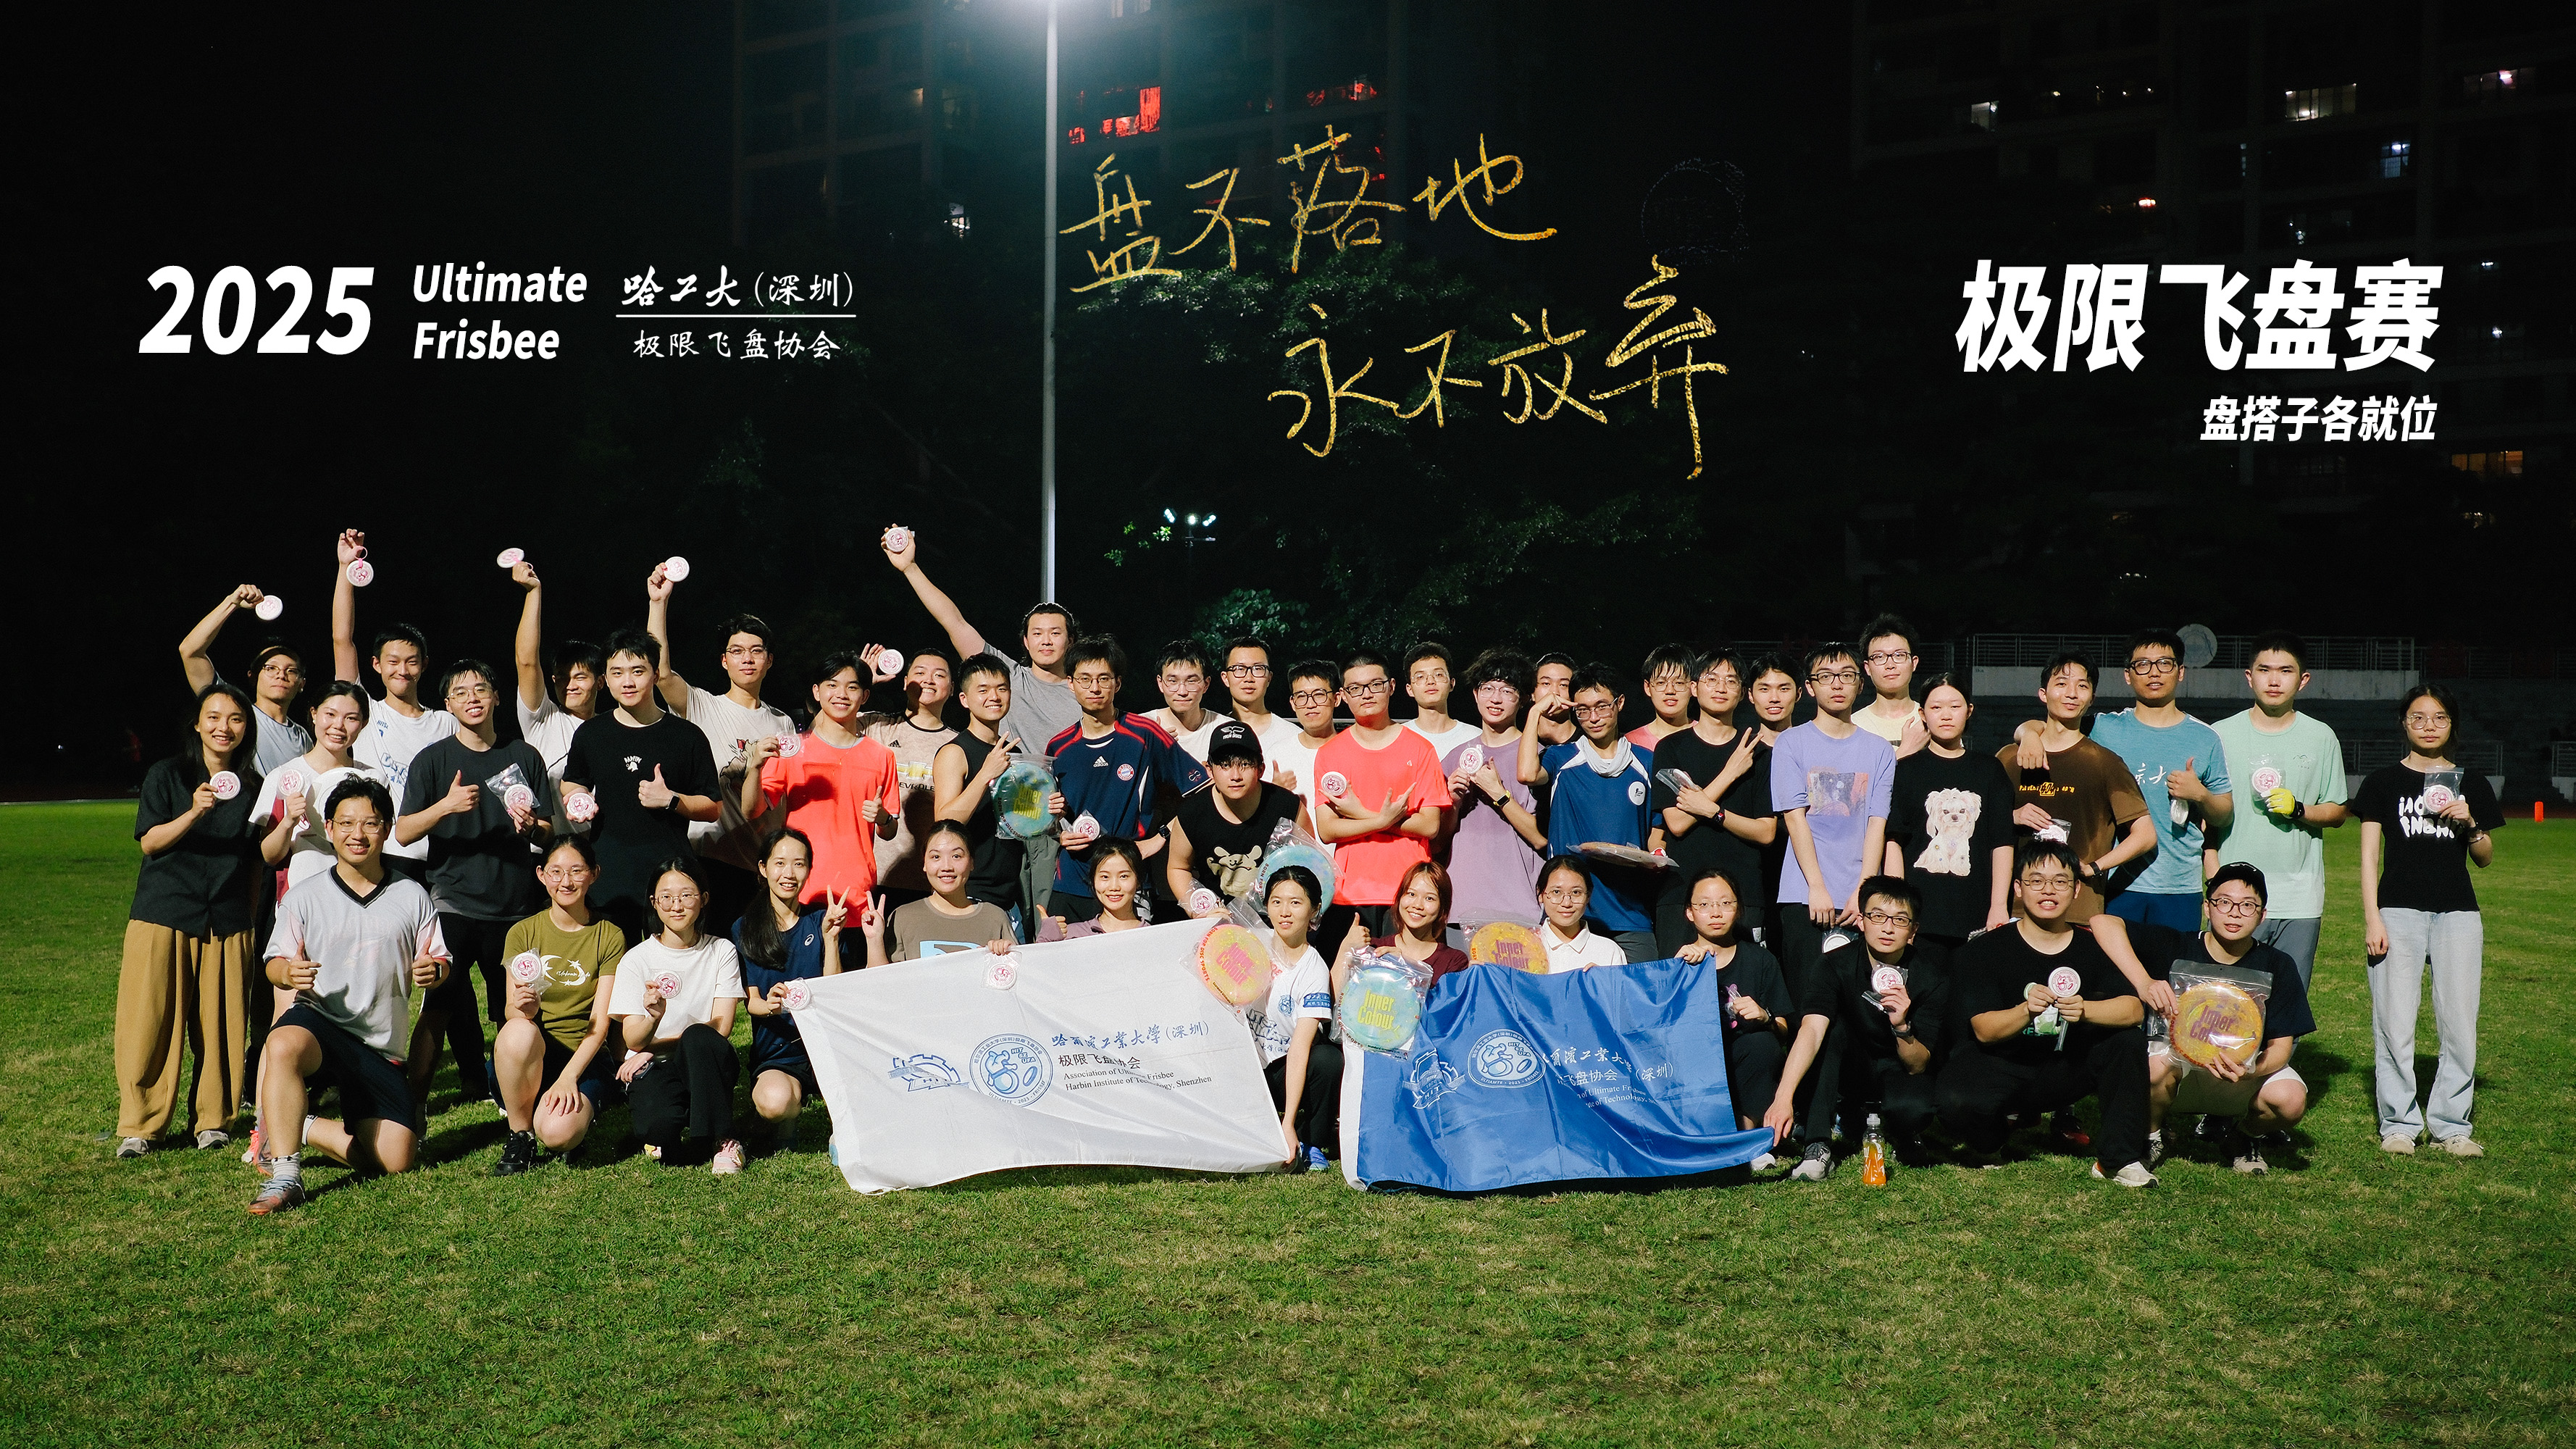
\includegraphics[width=\paperwidth, height=0.4\paperheight, keepaspectratio]{大合照.jpg}%
    % 或者使用 height=0.6\textheight,并根据是否需要保持宽高比决定 keepaspectratio

    % \vspace{0.5em} % 图片与彩色条带之间的可选间距

    % 彩色条带 (无文字,宽度为 paperwidth)
    \vspace{-1pt} % 此行用于消除图片和彩带间的微小间距,应保留
    \noindent\hspace*{-1in}%
    \colorbox{MyBannerTeal}{% % 使用您最终确定的颜色名称
        \begin{minipage}[c][2em][c]{\dimexpr\paperwidth-2\fboxsep\relax} % 彩色条带高度,例如3em,宽度为paperwidth
            \hspace{0pt} % 确保minipage有内容以正确计算高度
        \end{minipage}%
    }

    % 彩色条带下方的文本信息
    \begin{center}
        \vspace{4em} % 彩色条带与主标题之间的间距
        {\LARGE 2025年哈尔滨工业大学(深圳)体育文化节极限飞盘赛\par} % 主标题移到此处
        
        \vspace{1.5em} % 主标题与副标题之间的间距
        {\Large 赛程安排与注意事项 (5月30日, 6月4日, 6月6日)} \\[2em] % 副标题
        
        {哈尔滨工业大学(深圳)极限飞盘协会} \\[1em]
        {2025年5月21日}\par % 您可以按需更改此日期为实际发布日期

        \vspace{12em} % 在日期和旗帜之间添加一些垂直间距
        % 插入修剪后的协会旗帜 PDF
        % 您需要仔细调整 trim 的四个值 (左 下 右 上) 来正确修剪您的 PDF 旗帜。
        % 单位可以是 bp, pt, cm, in 等。
        % 例如: trim=10bp 20bp 10bp 20bp
        % width 可以调整旗帜显示的大小。
        
\includegraphics[width=0.65\paperwidth, trim=50bp 6.4cm 50bp 6.3cm, clip]{协会旗帜.pdf}
    \end{center}

    \vfill % 填充剩余垂直空间,或将底部内容推到底部(如果页面有足够空间)
\end{titlepage}

\clearpage
\pagenumbering{roman}
\pagestyle{plain}
\tableofcontents
\clearpage
\pagenumbering{arabic}
\pagestyle{fancy}

\section{赛事简介、赛制与场地说明}
本次极限飞盘赛采用4队小组循环赛加决赛轮的赛制,旨在为各队伍提供充分的交流和竞技机会。
\begin{itemize}
    \item \textbf{参赛队伍:} A队, B队, C队, D队。
    \item \textbf{小组循环赛:} 所有队伍两两之间进行一场比赛,共三轮比赛,每队参与三场。
    \item \textbf{比赛用时与规则:}
        \begin{itemize}
            \item \textbf{小组赛:}每场比赛时长50分钟,采用“抢10分”规则。
            \item \textbf{决赛轮:}每场比赛时长60分钟,采用“抢10分”规则。
        \end{itemize}
    \item \textbf{比赛信号:} 比赛开始与结束时,将以汽笛鸣一声为信号。
    \item \textbf{排位规则:} 小组循环赛(共三轮)结束后,根据各队积分进行排名。小组赛积分规则为:胜一场积2分,平一场积1分,负一场积0分。若积分相同,则依次比较:1) 相互间胜负关系(仅当两队同分时适用);2) 总净胜分(所有小组赛比赛的总得分数减去总被得分数);3) 总得分数。
    \item \textbf{决赛轮对阵:} 根据小组赛排名,进行如下对阵:
    \begin{itemize}
        \item \textbf{冠军赛:}小组赛第1名 vs 小组赛第2名
        \item \textbf{季军赛:}小组赛第3名 vs 小组赛第4名
    \end{itemize}
    \item \textbf{队伍颜色:} 为确保比赛中队伍区分清晰,每场比赛将为对阵双方指定深/浅色队服(通常第一个列出的队伍为深色,第二个为浅色,具体见赛程表)。请所有参赛队员务必\textbf{准备好深色(建议为黑色或深蓝色)和浅色(建议为白色)运动上衣各一件},并根据每场赛程安排穿着。
    \item \textbf{比赛地点与场地安排:}
    \begin{itemize}
        \item \textbf{比赛地点:} 哈工大操场。
        \item \textbf{场地设置:} 本次比赛将使用操场上的两个场地同时进行:
            \begin{itemize}
                \item \textbf{场地1:} 位于靠近维也纳酒店一侧。
                \item \textbf{场地2:} 位于远离维也纳酒店一侧。
            \end{itemize}
        \item \textbf{场地指引:} 请各队伍根据赛程表提前到达指定场地进行热身和赛前准备。
    \end{itemize}
\end{itemize}
\vspace{1em}
以下是本次体育文化节极限飞盘赛中三次活动的具体安排。请大家仔细阅读对应日期的安排,准时参加,注意安全,享受比赛!

\newpage

\section{第一比赛日:2025年5月30日(周五)- 小组循环赛 (第1、2轮)}

\subsection*{赛程安排 (5月30日)}
\renewcommand{\arraystretch}{1.8} % 增加行高使表格更疏朗
\begin{tabularx}{\textwidth}{@{} L{2.2cm} L{1.5cm} X L{3.2cm} @{}}
    \toprule
    \textbf{时间段} & \textbf{场地} & \textbf{对阵双方 (左队深色, 右队浅色)} & \textbf{阶段 / 备注} \\
    \midrule
    \multicolumn{4}{l}{\textit{20:00 - 20:10 到达、集合、队长报到、赛前准备、猜盘选边}} \\
    \addlinespace
    \multicolumn{4}{c}{\textbf{第一轮小组赛}} \\
    20:10 - 21:00 & 场地1 & A队 (深) vs C队 (浅) & 小组赛 - 抢10分 \\
    20:10 - 21:00 & 场地2 & B队 (深) vs D队 (浅) & 小组赛 - 抢10分 \\
    \addlinespace
    \multicolumn{4}{l}{\textit{21:00 - 21:10 中场休息、合影留念、换场准备}} \\
    \addlinespace
    \multicolumn{4}{c}{\textbf{第二轮小组赛}} \\
    21:10 - 22:00 & 场地1 & A队 (深) vs D队 (浅) & 小组赛 - 抢10分 \\
    21:10 - 22:00 & 场地2 & B队 (深) vs C队 (浅) & 小组赛 - 抢10分 \\
    \addlinespace
    \multicolumn{4}{l}{\textit{22:00 - 22:15 Circle交流、大合影}} \\
    \addlinespace
    \bottomrule
\end{tabularx}
\renewcommand{\arraystretch}{1.0}

\subsection*{当日重要提醒 (5月30日)}
\begin{itemize}
    \item 请所有队伍于 19:50 前到达总场地签到、热身。
    \item \textbf{重要服装提示:} 本日比赛颜色分配请严格参照上表,左队深色,右队浅色。
\end{itemize}

\newpage % 确保赛果和排名在新的一页

\section{第一比赛日赛果与积分排名 (截至5月30日)}

\subsection*{第一比赛日 (5月30日) 赛果}
\begin{itemize}
    \item \textbf{第一轮小组赛:}
    \begin{itemize}
        \item A队 9 -- 7 C队
        \item B队 7 -- 9 D队
    \end{itemize}
    \item \textbf{第二轮小组赛:}
    \begin{itemize}
        \item A队 10 -- 3 D队
        \item B队 5 -- 9 C队
    \end{itemize}
\end{itemize}

\subsection*{当前积分与排名 (截至5月30日赛后)}
\renewcommand{\arraystretch}{1.3}
\begin{tabularx}{\textwidth}{@{} M{1.2cm} M{1.2cm} M{1cm} M{1cm} M{1cm} M{1.2cm} M{1.5cm} M{1.5cm} M{1.5cm} @{}}
    \toprule
    \textbf{排名} & \textbf{队伍} & \textbf{场次} & \textbf{胜} & \textbf{负} & \textbf{积分} & \textbf{总得分} & \textbf{总失分} & \textbf{净胜分} \\
    \midrule
    1 & A队 & 2 & 2 & 0 & 4 & 19 & 10 & +9 \\
    2 & C队 & 2 & 1 & 1 & 2 & 16 & 14 & +2 \\
    3 & D队 & 2 & 1 & 1 & 2 & 12 & 17 & -5 \\
    4 & B队 & 2 & 0 & 2 & 0 & 12 & 18 & -6 \\
    \bottomrule
\end{tabularx}
\renewcommand{\arraystretch}{1.0}
\vspace{0.5em} % 增加一点垂直间距
\textit{注:C队与D队同积2分,两队尚未直接交手,比较总净胜分,C队(+2)优于D队(-5)。}

\newpage

\section{第二比赛日:2025年6月4日(周三)- 小组循环赛 (第3轮)}

\subsection*{赛程安排 (6月4日)}
\renewcommand{\arraystretch}{1.8}
\begin{tabularx}{\textwidth}{@{} L{2.2cm} L{1.5cm} X L{3.2cm} @{}}
    \toprule
    \textbf{时间段} & \textbf{场地} & \textbf{对阵双方 (左队深色, 右队浅色)} & \textbf{阶段 / 备注} \\
    \midrule
    \multicolumn{4}{l}{\textit{20:30 - 20:55 到达、集合、队长报到、赛前准备、猜盘选边}} \\
    \addlinespace
    \multicolumn{4}{c}{\textbf{第三轮小组赛}} \\
    20:55 - 21:45 & 场地1 & A队 (深) vs B队 (浅) & 小组赛 - 抢10分 \\
    20:55 - 21:45 & 场地2 & C队 (深) vs D队 (浅) & 小组赛 - 抢10分 \\
    \addlinespace
    \multicolumn{4}{l}{\textit{21:45 - 22:00 Circle交流、计算最终排名、场地整理}} \\
    \addlinespace
    \bottomrule
\end{tabularx}
\renewcommand{\arraystretch}{1.0}

\subsection*{当日重要提醒 (6月4日)}
\begin{itemize}
    \item 请所有队伍于 20:30 前到达总场地签到、热身。
    \item \textbf{重要服装提示:} 本日比赛颜色分配请严格参照上表,左队深色,右队浅色。
    \item 小组赛全部结束后将计算最终排名并公布决赛对阵。
\end{itemize}

\newpage

\section{第二比赛日赛果与小组赛最终积分排名 (截至6月4日)}

\subsection*{第三轮小组赛 (6月4日) 赛果}
\begin{itemize}
    \item A队 4 -- 9 B队
    \item C队 8 -- 10 D队
\end{itemize}

\subsection*{小组赛最终积分与排名 (截至6月4日赛后)}
\renewcommand{\arraystretch}{1.3}
\begin{tabularx}{\textwidth}{@{} M{1.2cm} M{1.2cm} M{1cm} M{1cm} M{1cm} M{1.2cm} M{1.5cm} M{1.5cm} M{1.5cm} @{}}
    \toprule
    \textbf{排名} & \textbf{队伍} & \textbf{场次} & \textbf{胜} & \textbf{负} & \textbf{积分} & \textbf{总得分} & \textbf{总失分} & \textbf{净胜分} \\
    \midrule
    1 & A队 & 3 & 2 & 1 & 4 & 23 & 19 & +4 \\
    2 & D队 & 3 & 2 & 1 & 4 & 22 & 25 & -3 \\
    3 & C队 & 3 & 1 & 2 & 2 & 24 & 24 & 0 \\
    4 & B队 & 3 & 1 & 2 & 2 & 21 & 22 & -1 \\
    \bottomrule
\end{tabularx}
\renewcommand{\arraystretch}{1.0}
\vspace{0.5em} % 增加一点垂直间距
\textit{注:}\\
\textit{1. A队与D队同积4分,小组赛中A队以10-3战胜D队,故A队排名靠前。}\\
\textit{2. C队与B队同积2分,小组赛中C队以9-5战胜B队,故C队排名靠前。}

\newpage

\section{第三比赛日:2025年6月6日(周五)- 决赛轮与颁奖}

\subsection*{赛程安排 (6月6日)}
\renewcommand{\arraystretch}{1.8}
\begin{tabularx}{\textwidth}{@{} L{2.2cm} L{1.5cm} X L{3.2cm} @{}}
    \toprule
    \textbf{时间段} & \textbf{场地} & \textbf{对阵双方 (左队深色, 右队浅色)} & \textbf{阶段 / 备注} \\
    \midrule
    \multicolumn{4}{l}{\textit{20:00 - 20:10 到达、集合、队长报到、决赛准备、猜盘选边}} \\
    \addlinespace
    \multicolumn{4}{c}{\textbf{决赛轮}} \\
    20:10 - 21:10 & 场地1 & A队 (深) vs D队 (浅) & \textbf{冠军赛} - 抢10分 (60分钟) \\
    20:10 - 21:10 & 场地2 & B队 (深) vs C队 (浅) & \textbf{季军赛} - 抢10分 (60分钟) \\
    \addlinespace
    \multicolumn{4}{l}{\textit{21:10 - 21:30 Circle交流、选取MVP、颁奖、大合影}} \\
    \addlinespace
    \bottomrule
\end{tabularx}
\renewcommand{\arraystretch}{1.0}

\subsection*{当日重要提醒 (6月6日)}
\begin{itemize}
    \item 请所有队伍于 19:50 前到达总场地签到、热身。
    \item \textbf{重要服装提示:} 决赛轮队伍颜色将根据实际对阵的队伍情况,在排名确定后现场协调或提前通知。
    \item 决赛轮对阵名单已根据小组赛最终排名确定。
\end{itemize}

\newpage % 确保新章节从新的一页开始

\section{决赛轮赛果与最终排名 (6月6日)}

\subsection*{决赛轮赛果}
\begin{itemize}
    \item \textbf{冠军赛:} A队 9 -- 8 D队
    \item \textbf{季军赛:} B队 10 -- 5 C队
\end{itemize}

\subsection*{最终赛事排名}
\begin{enumerate}
    \item \textbf{冠军:} A队
    \item \textbf{亚军:} D队
    \item \textbf{季军:} B队
    \item \textbf{殿军:} C队
\end{enumerate}

\subsection*{赛事MVP}
\begin{itemize}
    \item \textbf{A队 MVP:} 
        \begin{itemize}
            \item 张鑫 (2024312683, 清华深圳研究生院)
            \item 王肖辉 (2436194047, 北大深圳研究生院)
        \end{itemize}
    \item \textbf{B队 MVP:} 
        \begin{itemize}
            \item 李慧城 (2024312115)
            \item 欧阳笑琪 (清华深圳研究生院)
        \end{itemize}
    \item \textbf{C队 MVP:} 
        \begin{itemize}
            \item 刘慕实 (研0)
            \item 潘秀丽 (2024312180)
        \end{itemize}
    \item \textbf{D队 MVP:} 
        \begin{itemize}
            \item 朱乾坤 (24S153147)
            \item 周冰莹 (1701212988, 北大深圳研究生院)
        \end{itemize}
\end{itemize}

\newpage

\section{赛事总体注意事项}
\begin{enumerate}[label=\arabic*., itemsep=0.5em]
    \item \textbf{参赛服装:} 为配合赛事安排,请所有参赛队员务必为所有比赛日\textbf{各准备深色(建议为纯黑、深蓝等无明显花纹的暗色)和浅色(建议为纯白或其他无明显花纹的亮色)运动上衣各一件}。每场比赛的具体颜色分配请严格参照赛程表或听从现场指引。
    \item \textbf{饮水:} 场地不提供一次性水杯,请各位选手\textbf{务必自带充足饮用水及水壶}。
    \item \textbf{安全第一:} 请大家在比赛中务必注意自身和他人的安全,热身充分,量力而行,避免受伤。如有不适立即停止比赛并告知组委会。
    \item \textbf{保险:} 请所有运动员务必提前购买一日运动保险,组委会将随机进行抽查,没有购买保险的同学\textbf{不允许参赛},请务必知悉!
    \item \textbf{准时与场地:} 请各队严格遵守比赛时间,提前到场准备。如对场地位置不熟悉,请提前查看。
    \item \textbf{体育精神:} 秉持“Spirit Of The Game (SOTG)”飞盘精神,尊重比赛,尊重对手,尊重队友,公平竞争,享受运动。
    \item \textbf{场地保持:} 请爱护场地设施,比赛结束后自觉清理并带走各自产生的垃圾,保持场地整洁。
    \item \textbf{赛制理解:} 请各队队长及队员仔细阅读赛事简介与赛制说明,如有疑问可提前咨询组委会。
    \item \textbf{天气预案:} 如遇极端恶劣天气不适宜比赛,组委会将尽早通知后续安排。
\end{enumerate}
\vspace{1.5em}

\begin{center}
期待大家的积极参与,预祝比赛顺利,玩得开心!
\end{center}
\vspace{1.5em}

\noindent\rule{\linewidth}{0.4pt}
\vspace{1em}

\begin{flushleft}
\textbf{主办单位:} \\
哈尔滨工业大学(深圳)团委 \\[1em]

\textbf{承办单位:} \\
哈尔滨工业大学(深圳)极限飞盘协会(筹)
\end{flushleft}

\appendix
\section{参赛人员名单}

\subsection*{A队}
\renewcommand{\arraystretch}{1.2}
\begin{tabularx}{\textwidth}{@{} L{3cm} M{2cm} X @{}}
    \toprule
    \textbf{姓名} & \textbf{性别} & \textbf{学号} \\
    \midrule
    唐吉昕 & 男 & 24S055012 \\
    耿增越 & 男 & 2023311226 \\
    马悠然 & 男 & 2023311228 \\
    郑伟 & 男 & 24S153075 \\
    郝宇鑫 & 男 & 355012 \\
    刘尊 & 男 & 24S152072 \\
    倪梓源 & 男 & 2023313729 \\
    吴晓泽 & 男 & 2023311221 \\
    张毓芷 & 女 & 24S153036 \\
    冯思雨 & 女 & 24S053012 \\
    王婧璇 & 女 & 24s153138 \\
    张鑫 & 男 & 2024342683 \\
    王肖辉 & 女 & 2436194047 \\
    谢雯怡 & 女 & 19S054034 \\
    \bottomrule
\end{tabularx}

\subsection*{B队}
\renewcommand{\arraystretch}{1.2}
\begin{tabularx}{\textwidth}{@{} L{3cm} M{2cm} X @{}}
    \toprule
    \textbf{姓名} & \textbf{性别} & \textbf{学号} \\
    \midrule
    李明柠 & 男 & 2023311423 \\
    彭欧 & 男 & 220810335 \\
    陈昱 & 男 & 24S153084 \\
    刘证涛 & 男 & 2024311417 \\
    朱一辰 & 男 & 24S053027 \\
    黎骁 & 男 & 24S153047 \\
    武卓星 & 女 & 2024312707 \\
    刘玉姬 & 女 & 24S153097 \\
    邓智鸿 & 男 & 24S152054 \\
    李慧城 & 男 & 2024312115 \\
    李芝玘 & 女 & 24S053041 \\
    王硕 & 男 & 暂未入学 \\
    赵普洁 & 女 & 23B353001 \\
    吴承沣 & 男 & 23B353007 \\
    \bottomrule
\end{tabularx}
\renewcommand{\arraystretch}{1.0}

\subsection*{C队}
\renewcommand{\arraystretch}{1.2}
\begin{tabularx}{\textwidth}{@{} L{3cm} M{2cm} X @{}}
    \toprule
    \textbf{姓名} & \textbf{性别} & \textbf{学号} \\
    \midrule
    罗梦恬 & 女 & 2023311801 \\
    刘俊青 & 男 & 2401212419 \\
    徐浩文 & 男 & 24S153112 \\
    黄家骏 & 男 & 2024311040 \\
    罗模煊 & 男 & 2023311101 \\
    赵铭烁 & 男 & 2023316101 \\
    杨鸿鑫 & 男 & 2024312706 \\
    马睿政 & 男 & 24S153135 \\
    蔡俊 & 男 & 24B953040 \\
    蔚旺 & 男 & 24S153107 \\
    原子涵 & 女 & 24S053024 \\
    徐紫嫣 & 女 & 24S153142 \\
    潘秀丽 & 女 & 2024312180 \\
    黄佳乐 & 男 & 20233113 \\
    \bottomrule
\end{tabularx}

\subsection*{D队}
\renewcommand{\arraystretch}{1.2}
\begin{tabularx}{\textwidth}{@{} L{3cm} M{2cm} X @{}}
    \toprule
    \textbf{姓名} & \textbf{性别} & \textbf{学号} \\
    \midrule
    马煜捷 & 男 & 2023311A29 \\
    杨婧怡 & 女 & 23S055023 \\
    张文豪 & 男 & 24SF57248 \\
    蔡万金 & 男 & 224331403 \\
    蔡洛萱 & 女 & 2024314677 \\
    宁卓 & 男 & 24S043004 \\
    潘昱嘉 & 男 & 2023314227 \\
    张硕航 & 男 & 2024312309 \\
    赖正广 & 男 & 24S054005 \\
    朱乾坤 & 男 & 24S153147 \\
    李大壮 & 男 & 22S154170 \\
    李娅希 & 女 & 22S154146 \\
    邓嘉欣 & 女 & 24S153154 \\
    周冰莹 & 女 & 1701212988 \\
    \bottomrule
\end{tabularx}

\end{document}